\chapter{Crisis model distillation to extract actionable information from social media}

\section*{Introduction}
The context presented in the literature review highlighted the importance of information management during an emergency event.
Improving the response requires better coordination between the different actors.
However, a coordinated response can only be performed if all the partners easily share information.
The first chapter used the example of the Common Operational Picture (COP) as a visual medium for information sharing.
The COP makes it possible to display certain information with a vocabulary common to all actors.
However, this approach requires that all the actors agree beforehand on the information of interest.
During the preparation phase, COP is a way to create a shared Situational understanding between the different actors \parencite{steen-tveitCommonOperationalPicture2021}.
Also, the integration of information obtained from social media into this interface remains a challenge.
The previous chapter identified three aspects that could use a better information input using social media data:

\begin{itemize}
    \item Collaboration: the need for information to support coordination between partners
    \item Situational Awareness: the need for information that enables the identification of the elements that make up the environment
    \item Public communication: the need for information to understand the population's feelings regarding the event and facilitate public relations.
\end{itemize}

These needs are directly linked with the first sub-problem mentioned in the first chapter, namely: \emph{What decision-relevant information from social media can be processed automatically?}
The current chapter seeks to identify this relevant information to identify what could be automatically collected.
There are, therefore, at least two needs that must be considered: i) the information needs of decision-makers ii) the information required by the information system used to support the response.
As a result, the approach is twofold.
The first section considers the information needed from the point of view of a crisis management organization.
In particular, it identifies the profile of the people who deal with social media and the information sought.
This section is then based on the literature, meetings, and interviews with crisis management practitioners.
The second section focuses on previous crisis models proposed to digitalize crisis response.
These crisis models consist of abstract but automatable representations of the information during crisis management.
Thus, this section aims to identify the information needed to implement such models.
Finally, the third and last section is a conclusion that crosses the needs identified previously.
It presents the information that can be automatically handled by a computer to support decision-making.

\section{Information expected by practitioners}
This chapter thus draws on previous research and works realized alongside social studies conducted during the research project by social scientists.
This section is split into three parts.
The first part focuses on social media processing in crisis management organization.
It aims at answering the question \textit{Who is processing social media content in these organizations?}
The second part focuses on the information already identified in the literature.
Finally, the last part presents the first set of information corresponding to the information sought by decision-makers.

\subsection{Social media processing in crisis management organizations}
Crisis management organizations are composed of several actors with well-defined roles.
As the first chapter mentioned, crisis management involves multiple actors, and not all of them pay attention to social media content.
While decision-makers benefit from the insights coming from these platforms, they do not perform the collection themselves.
This section reports on the place of social media in different organizations observed in this study.
The research question that this part aims to answer is:
\emph{RQ: Who is in charge of social media handling in crisis response organizations?}
The observations and interviews with practitioners associated with previous results from the literature contribute to answering the previous RQ.

\subsubsection{Method}
The multidisciplinary and multicultural context of this study allowed to meet and exchange with a wide variety of crisis management actors.
This variety is welcome since, as presented in the next section, the treatment of social media in management knows no standard.
At least five occasions (summarized Table~\ref{table:terrain-summary}) provided valuable insights into the scope of the study.

\begin{table}[h]
    \centering
    \caption{Overview of the different meetings with practitioners.}
    \tabulinesep=1.2mm
    \begin{tabu} to \textwidth {X[1,m]X[2,m]X[0.8,m]}
        Occasion (Location)                    & Participants profiles                                                                                                                                          & Methodology          \\ [0.5ex]
        \toprule
        PSAPs Role Play (Charleston, SC)       & Call takers, Dispatchers                                                                                                                                       & Role-plays           \\[0.5ex]
        Early Adopters Summit (Charleston, SC) & 25 local 911 professionals (PSAPs Managers, Call-takers, Dispatchers, and IT technicians)                                                                      & Focus groups         \\[0.5ex]
        Exercise 1 MACIV (Var Départment)      & Professional and volunteer firefighters                                                                                                                        & Exercise observation \\[0.5ex]
        Exercise 2 MACIV (Vienne Department)   & The staff of the Prefecture 86, a communication officer, two representatives of the police, firefighters, and gendarmerie                                      & Exercise observation \\[0.5ex]
        Exercise 3 MACIV (South-West Zone)     & Southwest Zone and six of the twelve associated Préfectures (the 79, 47, 40, 17 ,23 , 87). The Préfectures had a similar composition as the one in exercise 2. & Exercise observation \\[0.5ex]
        \bottomrule
    \end{tabu}
    \label{table:terrain-summary}
\end{table}

% * Role-play
In the U.S., \textcite{graceRolePlayingNext2019} conducted role-plays at the Public-Safety Answering Point (PSAP) of Charleston (South Carolina).
This PSAP is tasked with answering calls from citizens and dispatching resources during emergencies.
The particularity of this PSAP is its adoption of a system allowing it to consider text messages (SMS) and reports from Internet platforms (social media) in addition to calls.
One of the objectives of these role-plays was to define with the call-takers and dispatchers what a perfect social media could be for them \parencite{kropczynskiIdentifyingActionableInformation2018}.
The study in the U.S. took place in the context of the development of Next-Generation 911.
As per the authors:
\blockquote{Next-Generation 911 (NG911) infrastructure will replace analog systems designed to support voice services for landline 911 callers with digital, IP-based systems that will allow smartphone users to "call" 911 via voice, text, image, and streaming video.}
The objective of these role-plays was to document how call center operators processed the incoming call to obtain information.
This study ultimately aimed to reflect this processing to social media messages.
This exercise highlighted many aspects of call center operations.
First, there are two types of operators who interact with information: call-takers and dispatchers.
Call-takers are responsible for receiving calls and getting the correct information from the callers.
The answers are shared with the dispatchers through the Computer-Aided Dispatch (CAD).
The CAD system allows for the entry of notes associated with the call.
The call-takers teams also use a CAD plugin called ProQA.
ProQA is an integrated expert system that provides a support function through question proposals and classifications for the event.
Protocols, as interpretive frameworks, shape information gathering and filtering.
The information pipeline in the case of the PSAPs was the following:

\begin{enumerate}
    \item A \textit{Caller} calls the PSAP through the 911
    \item The \textit{Call-taker} receives the phone call, asks questions to the Caller to obtain as much information as possible about the event.
          They then record their findings on the CAD system.
    \item The \textit{Dispatchers} receive an alert from the CAD that a new event is in progress. They then consult the notes provided by the call-takers to dispatch resources.
    \item The \textit{Responders} follow the instructions provided by the dispatcher to intervene on the scene of the incident.
\end{enumerate}

% * Early adopters summit
The 2019 911 Early Adopters' Summit provided the opportunity to meet 911 practitioners on the topic of NG911.
This summit was composed of many different profiles: managers of PSAPs, but also call-takers, dispatchers, and I.T. technicians.
The participants met during this event, as early adopters, were largely in favor of changes in emergency response.
\textcite{graceCommunicatingNextGeneration9112020} report their feelings and opinions through a Strengths-Opportunities-Weaknesses-Threats (SWOT) analysis \parencite{gaoConsolidatingSWOTAnalysis2011} on NG911.
The SWOT analysis lasted an afternoon and implied 25 participants, all of them being 911 professionals.
This type of analysis allows identifying of strengths and weaknesses (internal or external) of an organization.
The goal was then to reflect on these factors in the case of NG911 through the lens of this method.
The summit was also the occasion to capture the diversity of configurations of PSAPs that exist in the U.S.
Indeed, the setup documented during the Charleston role-plays is not standard, and each PSAP center is free to organize as it prefers.
So, depending on the constraints applied to the center, its structural organization might be different.
The call center can report to a remote dispatch center, along with other call centers, for instance.

% * Exercices MACIV
In France, the MACIV exercises were opportunities to observe how professionals respond in practice to a situation.
Figure~\ref{information:french-orga} illustrates the organization of the institutions in charge of the crisis response.
It is a hierarchical organization.
The hierarchy is based on the size of the area affected by the event.
The higher layer is the National level (not represented in the figure), then the Zonal level, the Départemental level, and the Communal level.

\begin{figure}[thb]
    \centering
    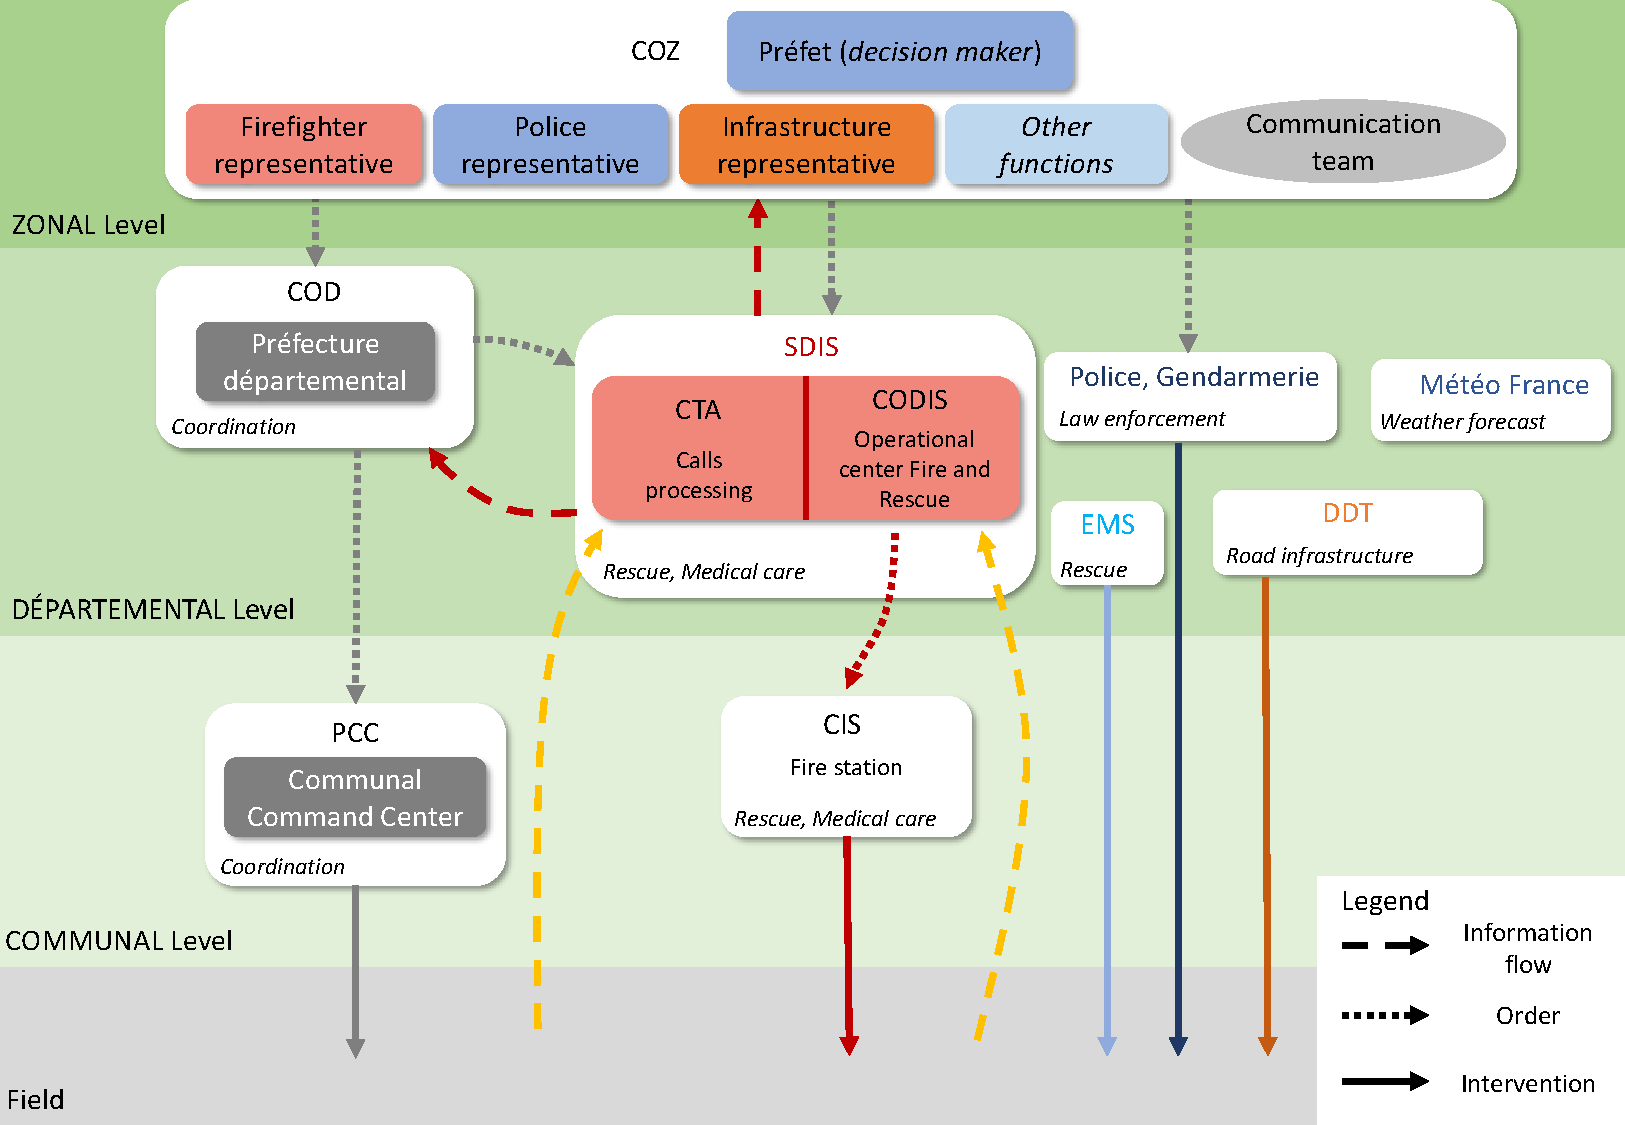
\includegraphics[width=\textwidth]{figures/chap-3/orga-gestion-crise.pdf}
    \caption{Diagram of the organization of the different French institutions involved during the response to an event of zonal scale. Illustration adapted from \textcite{batardIntegrerContributionsCitoyennes2021}}
    \label{information:french-orga}
\end{figure}

The Zonal and Départemental levels are governed by Préfectures (administrative institutions in charge of representing the government authority).
The services in charge of crisis response in these institutions are the Centre Opérationnel de Zone (COZ) and the Centre Opérationnel Départemental (COD).
The Départemental level also includes the highest representation of the response actors (firefighters, police, emergency services, etc.).
Among them, the Service Départemental d'Incendie et de Secours (SDIS, for \textit{Departmental Fire and Rescue Service}) oversees managing the rescue teams according to the priorities fixed by the COD.
The SDIS serves two functions: i) organized the rescue units and ii) handled phone calls.
The calls are handled through the Centre de Traitement des Appels (CTA, for \textit{Calls Processing Center}).
The organization and management of rescue teams is performed by the Centre Opérationnel Départemental d’Incendie et de Secours (CODIS).
The Centre Opérationnel de Zone provides instructions to the Centre Opérationnel Départemental or directly to the SDIS (see definition below).
The SDIS takes its orders from either the COZ or the COD.
It provides orders directly to the commanders of the units deployed or officers in charge of sub-centers—the CIS.
It receives back reports from the rescue teams and phone calls from victims.
They provide the information they have to the COZ and COD.
The last actor is the PCC, the crisis cell created in each Commune (the equivalent of Counties).

Another important player in these exercises was the VISOV association.
The Volontaires Internationaux en Soutien Opérationnel Virtuel (VISOV, French equivalent of the \textit{Virtual Operations Support Teams} — VOST) association is of volunteers.
These citizens organize themselves to help the institutional actors to identify the information related to an event posted on social media.
Their organization is further developed in \textcite[p.122--148]{batardIntegrerContributionsCitoyennes2021}.

The exercises involved three types of actors: an institutional actor, an association of volunteer citizens, and the research teams.
These exercises took place in the following manner.
First, the exercise was prepared and its characteristics set (role of each actor, choice of the type of crisis, actors involved according to their availability, etc.).
Then comes the exercise itself.
During the exercise, the institutional actors play their roles and address the event as they would normally do.
The VISOVs support the practitioners by processing the social media content provided for the exercise.
Finally, the research teams shadow the practitioners in their roles.
At the end of the exercise, an exchange phase allows the participants to give feedback on the exercise.
The main purpose of these exercises was to document the information flow within the French emergency management institutions, and particularly, the way information coming from social media was considered.
The types of events simulated were, respectively:

\begin{itemize}
    \item Flooding event in the Var Department at the Service Départemental d’Incendie et de Secours du Var (SDIS83).
    \item Snow event and consecutive traffic jam in the Vienne Department at the Vienne's Préfecture.
    \item Chemical incident in the South West of France involving the Southwest Zone and six of the twelve associated Préfectures (the 79, 47, 40, 17 ,23, 87) and the CODIS 47.
\end{itemize}

The three exercises were an opportunity to observe different institutions and the way they approach social media.
In the first exercise, social media were processed inside the SDIS83\footnote{Each French Department is associated with a number. In this case, the Var Department has the number 83}
by a Médias Sociaux en Gestion d'Urgence operator (MSGU, French equivalent of the \textit{Social Media in Emergency Management} — SMEM).
The setting of the SDIS is shown in Figure~\ref{information:exercice-1-setup}.
The decision-maker was a firefighter officer in charge of the room.
The officer was assisted by four firefighters managing the teams dispatched and their reports using a whiteboard.
One of the firefighters was taking phone calls from victims.
Directly to his right was a volunteer firefighter trained to gather social media information during the event.
Behind these two operators, a specialized volunteer firefighter was overseeing the cartographic desk.

\begin{figure}[htb]
    \centering
    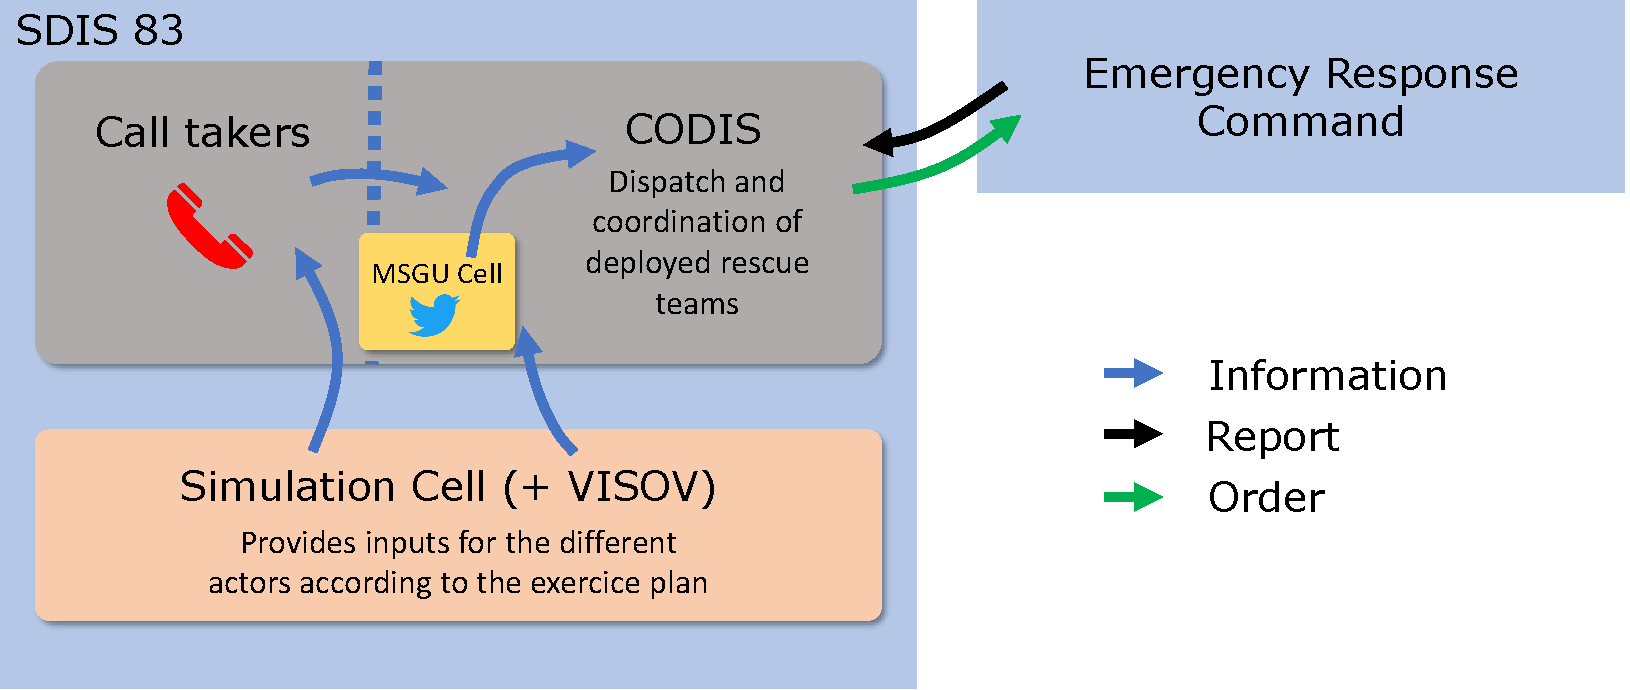
\includegraphics[width=\textwidth]{figures/chap-3/exercice-1-setup.pdf}
    \caption{Organizational diagram of Exercise 1 MACIV at SDIS83 in the Var Department. Illustration adapted from \textcite{batardIntegrerContributionsCitoyennes2021}.}
    \label{information:exercice-1-setup}
\end{figure}

The social media operator was who is familiar with social media and communication.
This operator was sharing a Google Sheet\footnote{https://www.google.fr/intl/fr/sheets/about/} document with the members of the VISOV association.
A Google Sheet document is a tabular file identic to an Excel file, where multiple persons can modify simultaneously the document and see the changes in real-time.
It is the possibility of having several actors collaborate in real-time on the same document that motivated the choice of this format.
The VISOV association is mostly composed of volunteers with a background in public service, rescue operations, etc.
These volunteers monitor social media on their own to identify information related to a potential or already ongoing event.
This operator was monitoring social media and cross-referencing the information they could obtain with that provided by the VISOV volunteers.
This live document is then shared with the person in charge of social media processing within official institutions.
Using their own findings and the ones from the online document, the MSGU operator will then provide the information obtained when asked by the decision-maker in the room.

The second exercise took place in the Vienne Département at the 86 Préfecture in Poitiers.
The institution studied was the Prefecture of Vienne through their COD and their communication cell Figure~\ref{information:exercice-2-setup}.
The COD was composed of a decision-maker (played by a subordinate of the Prefect), a person in charge of communication, two representatives of the police, the fire department, the gendarmerie, and other services (cartography, road infrastructures, etc.).
This institution uses software similar to the CAD software used in the U.S. to share information.
This information system is named SYNERGI (SYstème Numérique d’Échange, de Remontée et de Gestion des Informations).
The Prefecture did not have a dedicated social media handling service (MSGU) as in the first exercise.
Instead, the VISOV association volunteers transmitted their findings directly to the communication unit.
In this configure, the institution was more reliant on the processing realized by the VISOV association.
The operators in charge of the social media in the Préfectures were persons from the communication team of each Préfecture.
In this case, these persons were not familiar with emergency or rescue operations.
They were mostly tasked with communication to the public using the official accounts of the institution they were part of.
Monitoring of social media activity and information gathering were not the priorities of these operators.

\begin{figure}[htb]
    \centering
    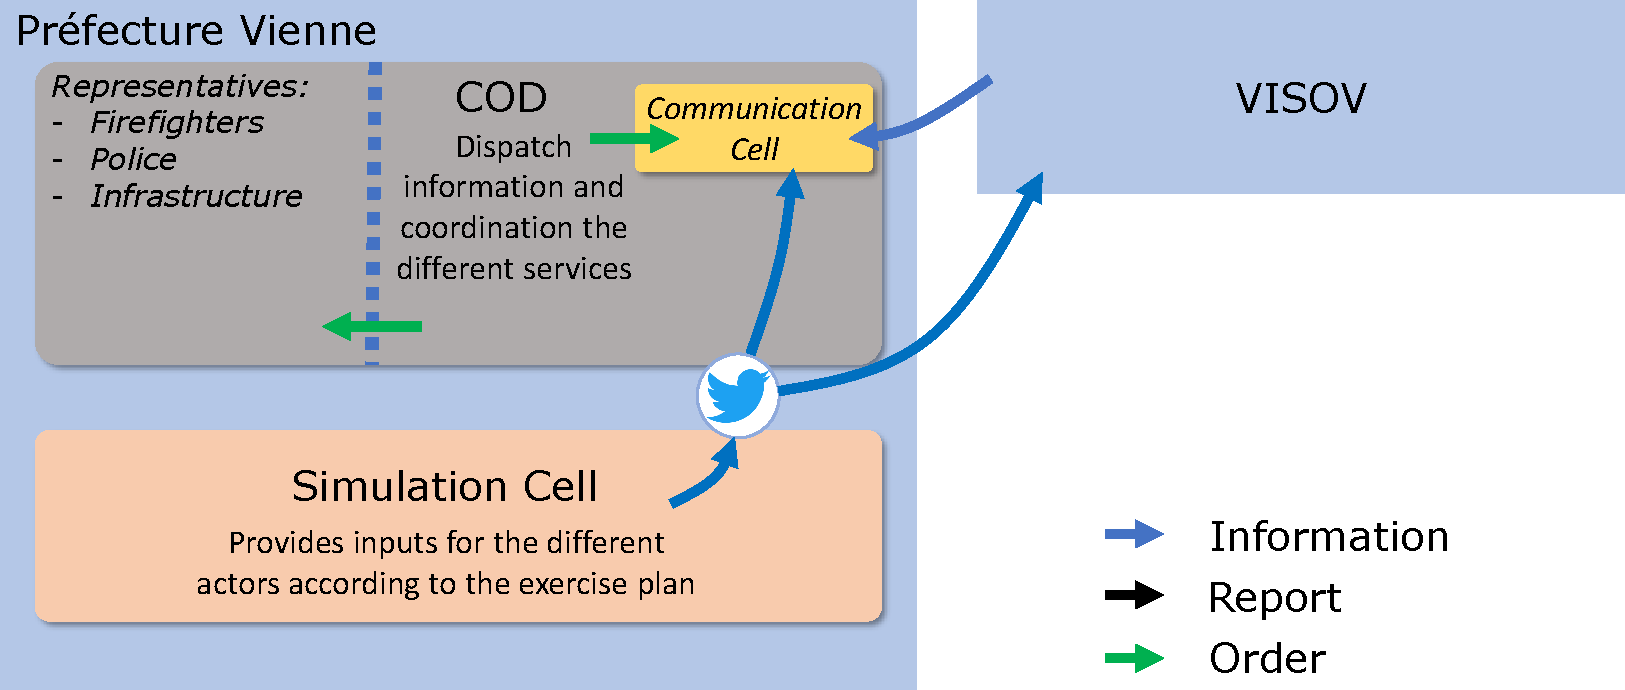
\includegraphics[width=\textwidth]{figures/chap-3/exercice-2-setup.pdf}
    \caption{Organizational diagram of Exercise 2 MACIV at the COD in the Vienne Department. Illustration adapted from \textcite{batardIntegrerContributionsCitoyennes2021}.}
    \label{information:exercice-2-setup}
\end{figure}

The third exercise saw similar actors involved but on a bigger scale.
Instead of one Préfecture, six were present under the direction of a Préfecture Zonal (see Figure~\ref{information:french-orga}).
The setting of this exercise is illustrated in Figure~\ref{information:exercice-3-setup}.
Each Préfecture involved the same organization as the second exercise (rescue team representatives, communication cell, specialized functions).
Similarly there was no MSGU cell created by the institutions.
As a result, they also relied on the VISOV association to obtain information from social media.
Also, the participating Préfectures were using the SYNERGI to exchange official information.

\begin{figure}[htb]
    \centering
    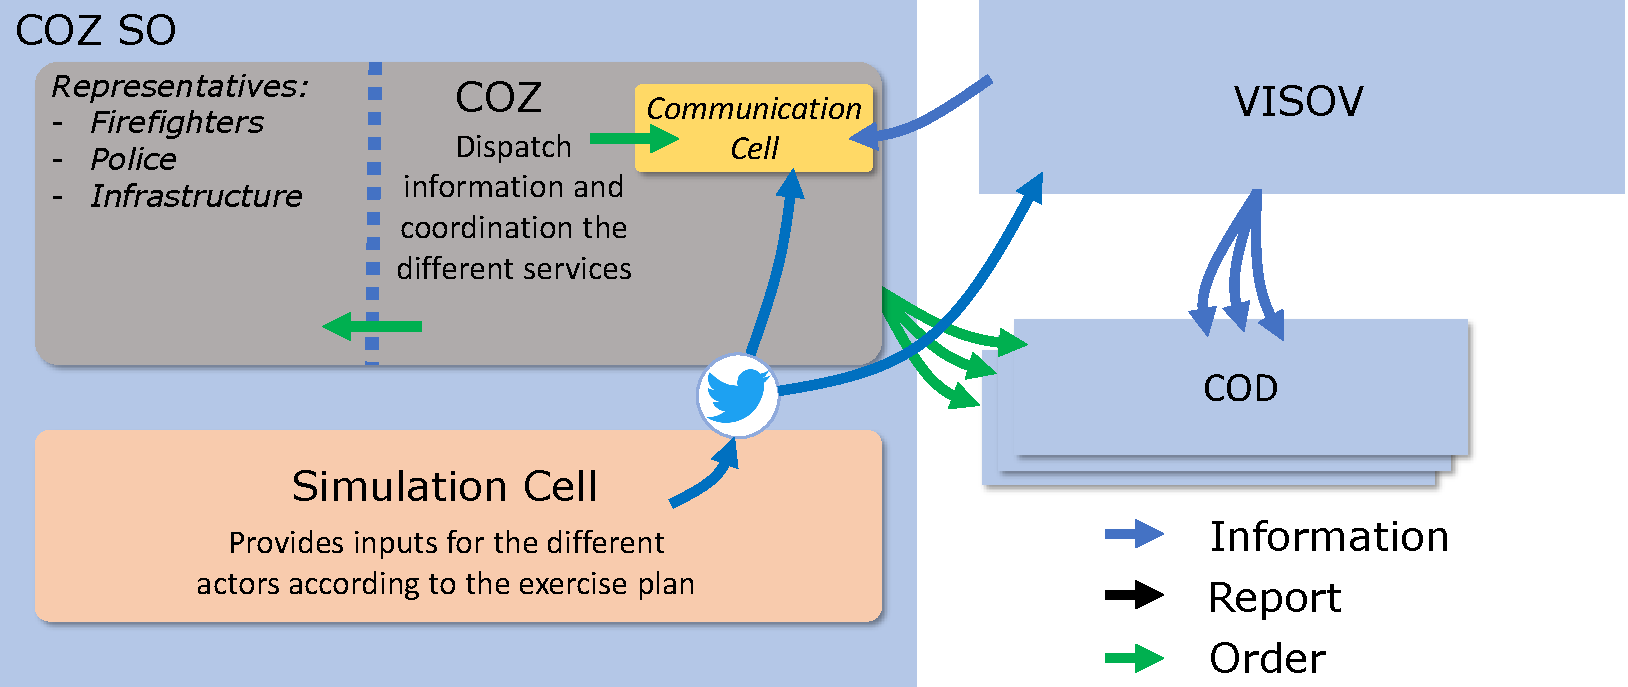
\includegraphics[width=\textwidth]{figures/chap-3/exercice-3-setup.pdf}
    \caption{Organizational diagram of Exercise 3 MACIV in the different Préfectures involved. Illustration adapted from \textcite{batardIntegrerContributionsCitoyennes2021}.}
    \label{information:exercice-3-setup}
\end{figure}

\subsubsection{Findings}
The various exchanges with the practitioners allowed us to understand better their functioning, their problems, and their overall feeling on the issue of social media.
The opportunity to carry out these observations in two different countries also allows us to understand better if some difficulties are local or shared between the two continents.
This section thus presents the key findings of these interviews.

\paragraph{A lack of tooling for processing social media content}
% * Done
The results of the SWOT analysis conducted during the Early Adopters Summit reveal that participants understand the value of this system.
Participants cite an improvement in the resilience of their information pipeline, thanks to the inclusion of new information channels such as social media that allow cross-checking the information obtained.
They also see NG911 as an opportunity to improve Situational Awareness of ongoing events.
On the other hand, participants noted concerns mostly related to the digitalization of their work environment.
Different platforms' volume, variety, and speed of data expose PSAPs to numerous threats such as misinformation and cybercriminals.
Participants also mentioned privacy issues.
The above threats require new protocols and tools for processing and new training for the personnel assigned to these new tasks.
However, all these new features come at a price, and the cost was identified as one of the main concerns about NG911.
Hence, social media processing systems, while they are wished by some practitioners, did not reach them yet.
Practitioners also find themselves struggling with the CAD system sometimes.
In the role-play conducted at the Charleston PSAP, \textcite{graceRolePlayingNext2019} reports that "the current system lacks flexibility. The operators reported 'breakdowns' in the information pipeline—corresponding to calls that do not provide the expected information or reported elements not relevant with an emergency."
Similarly, in France, the information system used in crisis response, SYNERGI, has some critics.
\textcite{linotPerspectiveComputationnelleDefi2018} report that the SYNERGI users suffer from:

\begin{itemize}
    \item Its rigidity, which leads to system circumvention.
    \item Communication issues, caused by a lack of common vocabulary.
    \item The diversity of unprepared institutions involved, leading to poor coordination.
    \item Lack of context associated with the information shared, adding confusion.
\end{itemize}

Also, the SYNERGI system prevents the collection or sharing of social media information on this platform.
The widespread use of the system and its official status hinders any rapid iteration of it.
The only integration of social media in an institution in France was during the first exercise.
But the system used was not official and was more like a homemade design that met a practical need.
Thus, it appears that the early adopters are unfortunately not so much.
Rather, they are individuals convinced of the value of social media in crisis management.
However, due to the lack of tools offering the necessary capabilities, it is difficult to consider this technology ready to enter the early adoption stage.
% Also, it is interesting to note the particular status of social media data within this information pipeline.
% \textcite{castagninoWhatCanWe2019} highlights the segregation of social media, systematically assumed as untrustworthy information during the first exercise.

\paragraph{Heterogeneous profiles of social media operators}
% * Done
The different sessions also allowed us to understand the diversity of profiles of people who deal with social media in crisis management.
The PSAPs encountered envisioned the role as an adaptation of call takers.
Thus, either an operator would be dedicated to social media monitoring, or existing call takers would be provided with an interface to monitor the content of interest.
In the past, when VOSTs were still in operation, some PSAPs (notably in the Colorado State) used these volunteers to assist them.
This third-party operation was found during the MACIV project exercises.
In France, media operators can be found at different levels in the hierarchy of response actors.
For the time being, this distribution depends on the interest that each one has in social media.
In the case of the first exercise, the SDIS had a dedicated operator alongside their call-taker and were cross-checking information.
In the other two exercises, it was the communication cell of the Prefectures that was monitoring social media to provide information to the decision-makers.
In all French cases, their operators were assisted by a third-party of volunteers, VISOV.
Overall, the processing of social media in crisis cells is carried out in a relatively similar manner in France and the U.S.
Both countries dedicated a person to the processing and kept this person in proximity with the decision-makers.
For instance, in France, the social media operator was in each exercise in the same room as the latter.
The organizations in charge of the response also rely (or have relied on) on a partner (the VISOV in France or the VOST in the U.S.).
Consequently, the processing is not always directly made by the social media operator present in the crisis cell.
Thus, there is currently one or more intermediaries between the fact and the decision-maker, as may be the case with telephone calls or reports made by response teams.
Gathering information from social can then be challenging because of the current lack of framing in the process of information collection.
Finally, the skill profile of the operators is also currently very diverse.
In France, the profiles observed were those of communicators, while in the United States, the people considered would be specially trained.
In the former case, these profiles translate a vision more oriented toward information dissemination rather than information collection.
As reported in \textcite{castagninoWhatCanWe2019}, French emergency organizations systematically assume information coming from social media as untrustworthy information.
Thus, for them, social media is more a communication channel than a collection channel.

\paragraph{Framing information collection: the Six Ws}
\label{sec:sixws}
% * Done
The Role-Play session at the Charleston PSAP brought interest in the way the information collection is framed by call-takers \parencite{kropczynskiIdentifyingActionableInformation2018}.
\blockquote{The "Six W's"—Where, What, Weapons, Who, When, and Why—provide call-takers with a heuristic for questioning callers and entering only relevant information for each call.}
The call-takers from the 911 PSAP's frame their interviews with the callers through the Six W's.
The goal of the Six W's is to obtain information that matches the information needs of the decision-makers.
These Six W's are:

\begin{itemize}
    \item \textit{Where} is the assistance needed,
    \item \textit{What} is the event taking place,
    \item \textit{Weapon(s)} involved in the event (if relevant to the nature of the event),
    \item \textit{Who} is involved in the event,
    \item \textit{When} the event started,
    \item \textit{Why} the event is happening.
\end{itemize}

These specific questions help the call-takers to acquire quickly detailed information relevant for decision-making.
This information was previously identified as the most relevant information to respond quickly and effectively to an emergency.

\subsection{A plurality of information needs in crisis management}
% * Done
It appears that in most cases, the information coming from social media passes through at least one intermediary before reaching the decision-maker.
Thus, while decision-makers need information, but they are not the persons actively monitoring social media.
The staff responsible for retrieving information from social media must therefore orient their research towards the needs of the latter.
Several questions therefore arise:

\begin{itemize}
    \item What information do decision-makers need?
    \item What information are the operators looking to retrieve?
\end{itemize}

The first question is at the heart of the crisis management system.
The decision-makers needs have to be answered, and this is the role of the support operators (call-takers and social media operators) to fulfill these needs.
The second question looks at the information that operators search for in the stream of social media messages.
This question guides the development of the algorithms responsible for retrieving data presented in the next chapter.
The remainder of this section develops the analysis of this need considering previous works that have defined concepts such as Situational Awareness and Actionable Information.

\subsubsection{Situational Awareness}
% * Done
\label{sec:situational-awareness}
Situational Awareness is summarized as the understanding of the "big picture" of a situation.
More precisely, it is the comprehension of the different aspects of an event, environment, and/or entities and how they are more likely to evolve in the near future.
Sufficient Situational Awareness is a critical factor in decision-making.
Each individual has their own Situational Awareness, depending on several factors such as experience, perception ability, training, etc.
The group formed by individuals also carries its Situational Awareness.
As described in Chapter 1, emergencies are confusing events that reset Situational Awareness.
The decision-makers in charge of the response must therefore build an updated mental representation of their environment.
This task is even more difficult as the context is unstable and may continue to evolve because of aftershocks or cascade effects.
In addition, the amount of new information can be overwhelming, depending on the size or complexity of the event.
In the described context, it appears crucial that decision-makers rely on adapted methodologies and tools to reconstruct adequate Situational Awareness for decision-making.
This work and definition attracted the interest of the U.S. military, who embraced the concept, working permanently in a stressful and highly uncertain environment.
\textcite{departmentofthearmyAdvancedSituationalAwareness2021} compiles the doctrine they have built around the concept, including how it fits into the decision-making process and how Situational Awareness is influenced by the environment.

The currently dominant definition is seminal work presented in \parencite{endsleyTheorySituationAwareness1995}.
\citeauthor{endsleyTheorySituationAwareness1995}, propose a definition of Situational Awareness as well as a model to explain how it fits into the decision-making process.
They define Situational Awareness as the:
\blockquote{perception of the elements in the environment within a volume of time and space, the comprehension of their meaning, and the projection of their status in the near future.}
This definition is associated with three levels: (1) perception, (2) comprehension, and (3) projection.
Perception refers to an operator's ability to detect relevant signals through its senses.
Level 2, comprehension, refers to the ability to interpret and make connections between the perceived signals.
Finally, level 3 corresponds to the ability to anticipate future events based on available information.
Figure~\ref{information:SA} provides an overview of Situational Awareness in the decision-making process according to \parencite{endsleyTheorySituationAwareness1995}.

\begin{figure}[htb]
    \centering
    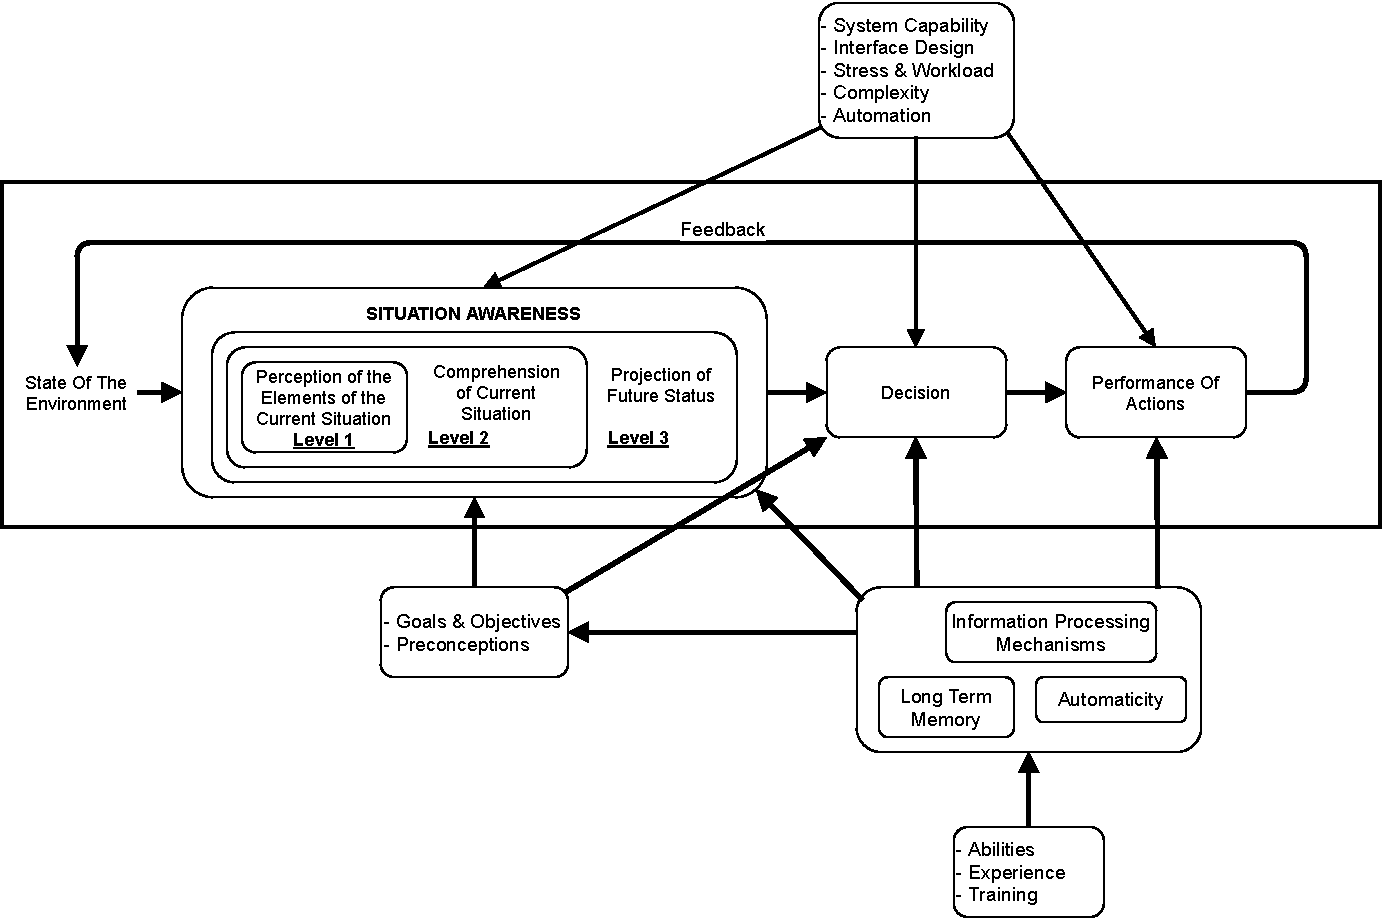
\includegraphics[width=\textwidth]{figures/chap-3/Endsley-1995.pdf}
    \caption{Adapted Situational Awareness model from \textcite{endsleyTheorySituationAwareness1995}.}
    \label{information:SA}
\end{figure}

Endsley's definition of Situational Awareness has seen many developments in the field of crisis computing.
Crisis models are one of these developments.
These computerized representations of the crisis terrain indeed meet the need for Situational Awareness.
For example, the model presented by \textcite{benabenMetamodelItsOntology2008} provides an interface representing the different actors and what they are doing, the components of the event, and the environment.
Later, \textcite{fertierRealtimeDataExploitation2020} proposed a system to automatically implement such models using sensors data to improve the Situational Awareness of its users.
\textcite{viewegSituationalAwarenessMass2012} uses the previous definition of Situational Awareness to propose a coding scheme for messages posted on social media.
This analysis highlighted that social media contain information that can improve Situational Awareness.
The automated extraction of messages contributing to Situational Awareness is then proposed in \textcite{vermaNaturalLanguageProcessing2011}.
Inspired by this proposition, many systems have been developed to classify messages according to certain categories of information \parencite{carageaClassifyingTextMessages2011, imranAIDRArtificialIntelligence2014,ashktorabTweedrMiningTwitter2014}.
More and more complex approaches are proposed.
For example, the processing is no longer limited to text only, but now also integrates the associated images \textcite{alamImage4ActOnlineSocial2017}.
The primary objective of this approach is to improve the classification results.
But aggregating data sources also allows providing the user with more points of view of the situation.
Having access to several data sources will also allow the user to cross-check the information from both channels to verify the information or complete certain aspects that would be missing on one of the channels.

\subsubsection{Actionable information}
% * Done
Interviews conducted with crisis managers and operators of call centers revealed a need for information other than situational awareness \parencite{zadeSituationalAwarenessActionability2018, kropczynskiIdentifyingActionableInformation2018}.
The interviewees refer to the need for actionable information, i.e., information that enables direct decision-making leading to a physical response.
During an event, a crisis management team can lack the critical information to take action.
This situation can arise when teams do not have the information they need to act or when they have to analyze a large volume of information.
This leads to a situation of paralysis of the decision-makers, despite the availability of the necessary information.
Situational Awareness is an important part of the decision-making process.
However, it does not specify what information is needed for the decision-making.
Systems that seek to improve Situational Awareness (e.g., by retrieving information posted on social media) do not guarantee that this information will be relevant to decision making.
Such an approach can even potentially contribute to the information overload mentioned above.
Hence, the proper design of these systems is of utmost importance (see Chapter 5).
The rest of this section focuses on this concept, its definition, and what it implies for the processing of social media data.

Actionable information can then be considered as a specific type of information.
\textcite{yangDesignPrinciplesIntegrated2012} indicate that the fire response system they propose should focus on information that is (i) timely, (ii) accurate, and (iii) complete.
For instance, information that provides the exact location of the event (accurate information) and the environmental conditions (complete information).
\textcite{comesBringingStructureDisaster2015} call for a similar set of attributes to define the information needed in an information system for crisis response: (i) relevant, (ii) accurate, (iii) timely.
\textcite{zadeSituationalAwarenessActionability2018} conducted a survey and various interviews of emergency and humanitarian responders.
They focused their research on the question: "how can the right information reach the right person at the right time?"
In their approach to this research, they first asked practitioners to define actionability.
They report:
\blockquote{participants described actionable information as anything which either they or their organization could use at that moment to assist, enact, or expedite the solution to a (potentially) identified issue.}
More importantly, the authors report that the practitioners use a different definition depending on their organizational role and responsibilities.
\citeauthor{zadeSituationalAwarenessActionability2018} identified the same attributes as the previous authors.
However, they also highlight the dependence of the definition of actionable information on the receiver of the information.
Thus, information may lead a particular type of decision-maker to decide.
In contrast, a decision-maker in charge of other aspects may judge the information provided as unimportant.
For instance, a piece of information can be actionable for firefighters but not for EMS.
The same authors also add the criteria of credibility.
Information that is not convincing will not lead to any response from the decision-makers.
As a result of all the points of view presented, a piece of information is actionable if it is:

\begin{itemize}
    \item Accurate: contains a location
    \item Addressed to the right role: the right decision-maker receives the information
    \item Timely: it reaches the decision-maker at the right time, e.g., avoiding a danger.
    \item Credible: it is considered
    \item Complete: it provides sufficient context on the environment.
\end{itemize}

\textcite{kropczynskiIdentifyingActionableInformation2018} relied on the Six W's previously presented to identify actionable information posted on social media.
The concept of actionable information is indeed at the heart of the Six W's, which seek to obtain the information necessary to make decisions.
The authors ,therefore, proposed to use the same approach for social media content.
Later, the same authors proposed a refined version of this coding scheme \parencite{kropczynskiRefiningCodingScheme2019}.
They conducted an analysis of a corpus of tweets to determine the appearance of actionable information in social media posts.
They coded 200 tweets using their proposed coding schema and reported the proportion of tweets that were fitting in these categories.
Their results show that among the tweets, four of the categories (Where, What, Who, Why) were significantly present, while two (Weapon and When) were rare.
With social media content, the Six W's might process is then slightly modified.
Usually, there is no follow-up information to fill the missing attributes like in a regular phone call.
A social media processing, therefore, must consider that specificity.
It can be addressed by aggregating the pieces of information retrieved from both call-takers and social media operators within a unified system.

\subsection{Location of Actionable Information in the Situational Awareness model}
% * Done
Situational Awareness is the initial building block of decision-making in crisis response.
Information cannot be designated as actionable without the decision-maker having sufficient context to decide if that information is actionable.
Therefore, crisis management starts by recovering an adequate perception of the elements/assets of the environment (level 1 of S.A.).
From that perception, they will use their skills/training to understand (level 2 of S.A.) the current situation.
Then, decision-makers evaluate the future status of their environment (level 3 of S.A.).
In this picture, Actionable Information is information that can trigger a decision or focus from the decision-makers.
This section aims to unify both concepts, starting from the Situation Awareness model.

Building Situational Awareness requires information and Actionable Information also depends on \textit{Information}.
Hence, both concept of Actionable Information and Situational Awareness relies on the definition of \textit{Information}.
Several definitions of \textit{Information} have been proposed.
\textcite{ackoffDataWisdom1989} proposed a hierarchical framework where four concepts, Data-Information-Knowledge-Wisdom, are used.
Later, \textcite{benabenMetamodelKnowledgeManagement2016} refined this framework to embed the concepts of \textit{Decision}.
Here, the definitions of \textit{Data} and \textit{Information} are only used.
The concept of \textit{Data} refers to symbols that have no meaning beyond their existence.
\textit{Information} is built from \textit{Data}, by structuring them.
Therefore, \textit{Information} is contextualized, organized, or structured \textit{Data}.
\textit{Information} generally answers questions such as "who," "what," "where," and "when."
Thus, the Call-takers interviewed in \textcite{kropczynskiIdentifyingActionableInformation2018} are gathering \textit{Information} through the Six W's.
The remaining part of this section presents an interpretation of the place of Data, Information, and Knowledge in Situation Awareness and the role of Actionable Information.
This interpretation is illustrated in Figure~\ref{information:SA-DIK}.

The first level of Situational Awareness described in \textcite{endsleyTheorySituationAwareness1995} concerns the perception of the "elements/assets" of the environment.
These "elements" or "assets" can correspond to images or text messages in the context of social media processing during crisis response.
This first step can thus be interpreted as the collection of \textit{Data} points.
These \textit{Data} are then processed and cross-referenced with each other, with the help of prior \textit{Knowledge}, to enable the understanding of the situation.
This step can therefore be seen as the beginning of the construction of \textit{Information} by the organization.
This is this level of Situational Awareness that decision-makers are required to reach to be able to decide.
Finally, the state of this \textit{Information} can be projected into the future to anticipate the future status of the environment and the event.
In this image, \textit{Knowledge}  intervenes in two places.
First, it allows the interpretation of \textit{Data} into \textit{Information}.
Second, it allows the projection resulting from the analysis of the \textit{Information}.

\begin{figure}[htb]
    \centering
    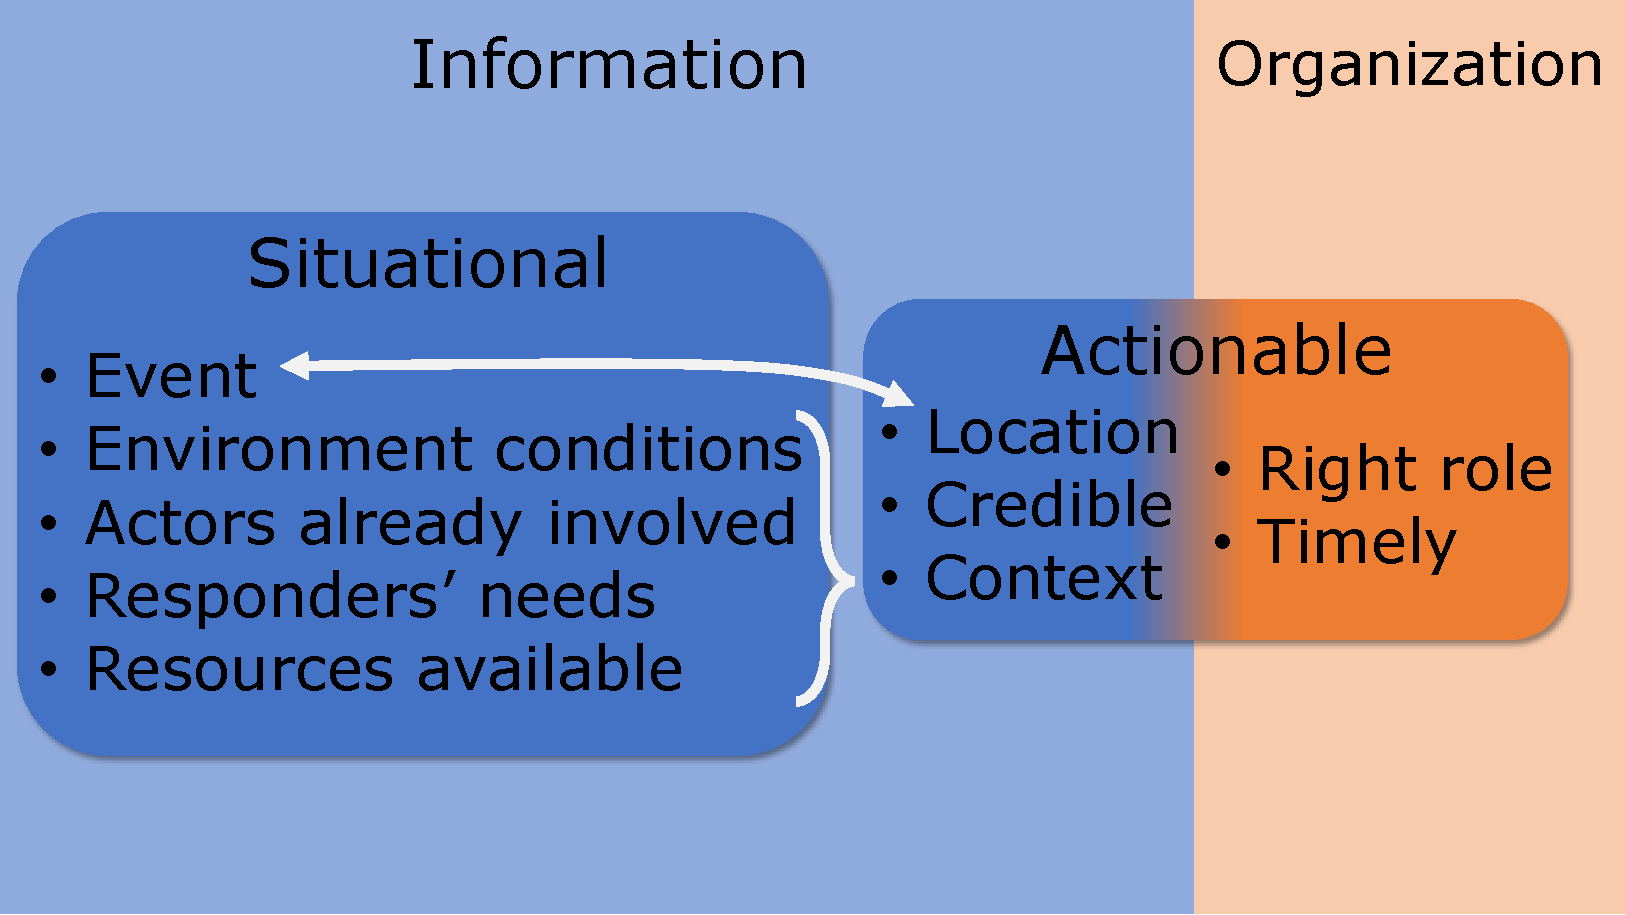
\includegraphics[width=\textwidth]{figures/chap-3/sa-actio-inf.pdf}
    \caption{Location of Data-Information-Knowledge concepts in the Situational Awareness model}
    \label{information:SA-DIK}
\end{figure}

Situational Awareness is built upon any \textit{Data} or \textit{Information} about the current state of an environment, and that is delivered to the decision-maker.
Using the previous proposition, we are now able to envision a relationship between Situational Awareness and Actionable Information.
As Actionable Information is a type of \textit{Information}, it is then embedded in the second level of Situational Awareness.
The difference with regular \textit{Information} is that Actionable Information is the missing piece of the puzzle that allows the decision-makers to decide.
As a result, Situational Awareness is the puzzle comprised of pieces of \textit{Information} that decision-makers try to assemble during the event.
Actionable Information constitutes the final, missing pieces of that puzzle necessary to comprehend the whole.
Actionable Information is then a specific piece of \textit{Information} in the Situational Awareness model.

\subsection{Information needs of a crisis management organization}
% * Done
This last section seeks to answer the question: \textit{What information do decision-makers need?}
The previous section showed that they need two types of information: information that improves their Situational Awareness and Actionable Information.
To provide a more concrete answer we rely on the results of the observations made during the research project as well as on the literature.
Figure~\ref{information:sa-inf} summarizes the relationship between Situational Awareness and Actionable Information.

Situational Awareness requires information about the event environment.
First, they need constant and specific information—What is the emergency? Where is the emergency? What are the conditions at the location?
Any information related to the event is potentially interesting.
However, to avoid overloading the teams with information, it may be advantageous to restrict the type of information sought.
\textcite{jacksonInformationSharingEmergency2006} thus proposes the following information to describe an event:

\begin{itemize}
    \item Location of event, type, cause, and severity.
    \item Environmental conditions (buildings, population density, potential hazards, and their location, etc.).
    \item Information on the response participants (responders already involved, their skills, resources, etc.).
    \item Current and future needs of the responders (number of casualties, their status, etc.).
    \item The available resources for the event (qualified actors, appropriate equipment, etc.).
\end{itemize}

This information is used to describe the context of the event.
This information also corresponds to the type of information that the Six W's are looking for.
\textcite{yangDesignPrinciplesIntegrated2012} also used this information in the design of their firefighting system.
In a second step, we also seek to obtain Actionable Information of interest to the crisis management teams.
Actionable Information is a piece, or the last missing piece, that enables decision-making.
As seen previously, Actionable Information is information that meets the following criteria, ordered by importance:

\begin{enumerate}
    \item is located;
    \item is directed to the right role;
    \item is timely;
    \item is credible;
    \item provides context.
\end{enumerate}

In addition, certain information allows for the de facto fulfillment of certain criteria.
For example, a message that mentions deployed units fulfills the context criterion.
Another example is a message that indicates the address of the event, thus fulfilling the location criterion while being a piece of information referring to an event.

\begin{figure}[htb]
    \centering
    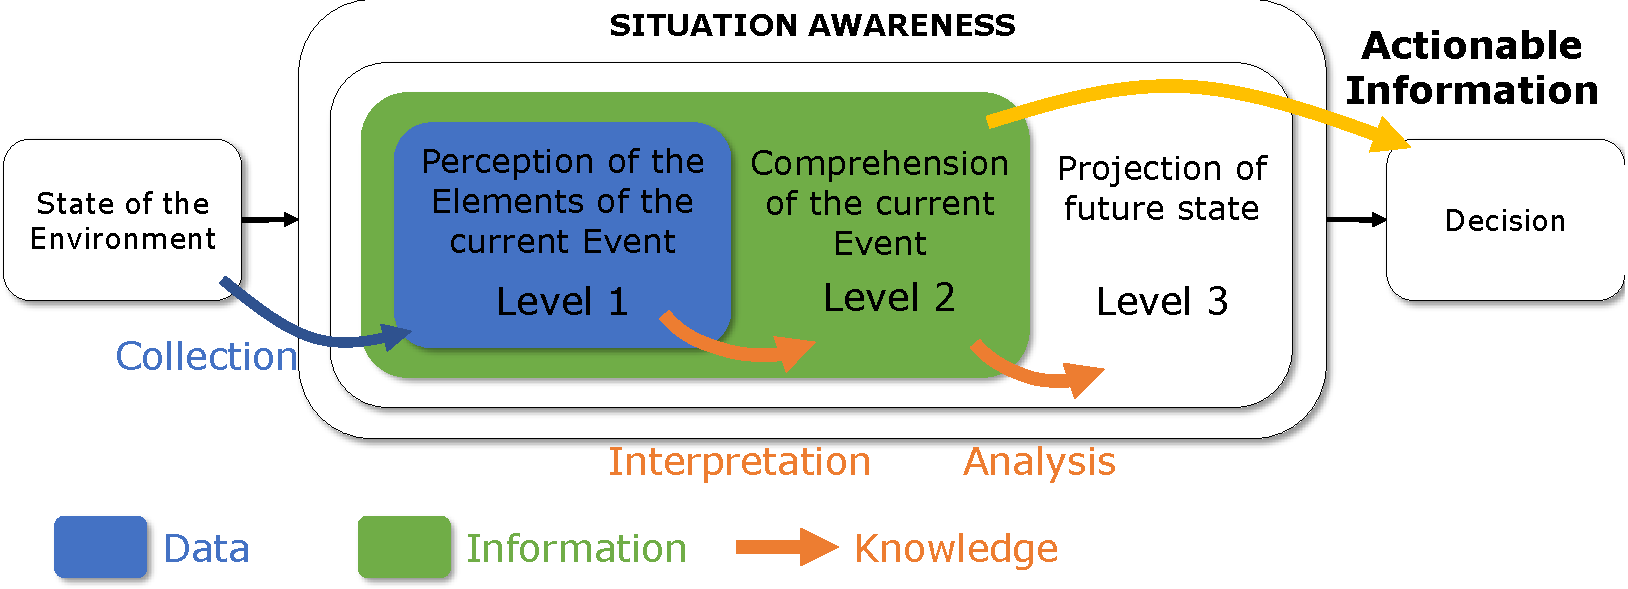
\includegraphics[width=\textwidth]{figures/chap-3/inf-need-dm.pdf}
    \caption{Information contributing to the Situational Awareness and criteria for a piece of information to be actionable and how they relate to each other.}
    \label{information:sa-inf}
\end{figure}

This section sought to answer two questions:

\begin{itemize}
    \item Who is processing social media during an event?
    \item What information do decision-makers need?
\end{itemize}

The first question was answered during the various meetings and observations of this research project.
Thus, it appears that decision-makers are not directly involved in social media processing.
This is done by dedicated operators, with various profiles that often correspond to the perception that organizations have of social media.
These operators then act as intermediaries between social media and the decision-maker.
The exploration of the second question showed that decision-makers use two types of information.
First, information that allows them to improve their Situation Awareness during the event.
Second, the need for Actionable Information, which allows for decision-making.
This section, therefore, concludes with a set of information that feeds the first need and a set of criteria that define whether an information is actionable.
The approach taken in this section can be characterized as bottom-up.
The next section takes the opposite approach, focusing on the needs identified for the design of information systems for crisis management.

\section{Information expected by information systems}
\label{sec:crisismetamodel}
The previous section consisted of a bottom-up approach to obtaining the information needed.
This section takes the opposite direction, i.e., top-down, starting from the need identified during the conceptualization of the crises and the information deemed necessary for the IT system.
As in the previous section, this approach also seeks to bring out a set of information relevant to crisis management.
The previous chapter (Chapter 2) provided a history of the information models developed for crisis management (section \hyperref[sec:lit-information-models]{2.2.1}).
These models provide a computer-readable representation of the information used by the different actors.
They then provide assistance through an information system that facilitates the distribution and manipulation of this information.
Two models are emerging in the context of improving collaboration between different crisis management actors \parencite{othmanDevelopmentValidationDisaster2014,benabenMetamodelItsOntology2008}.
\textcite{othmanDevelopmentValidationDisaster2014} propose four metamodels for disaster management, one for each phase of crisis management: mitigation, preparation, response, and recovery.
Their proposition is presented in Figure~\ref{information:othman-metamodel}.
Their model is constituted of four principal entities:

\begin{itemize}
    \item Disaster
    \item Rescue
    \item Emergency Management Team
    \item Response Organization
    \item Emergency Operation Center
\end{itemize}

An \textit{Emergency Operation Center} latter is a \textit{ResponseOrganization} that controls the \textit{EmergencyManagementTeam}.
A \textit{ResponseOrganization} is composed of groups of \textit{Aids} and \textit{Resources} at its disposal and is organized according to an \textit{EmergencyPlan}.
It supports the \textit{Rescue} teams in their efforts to rescue \textit{Victims} according to their \textit{Situational Awareness} and their \textit{Exposure} to the \textit{Disaster}.
The \textit{Rescue} teams are managed by an \textit{EmergencyManagementTeam}.
This team oversees defining a set of \textit{ResponseTask} according to given \textit{ResponseGoal}.
It follows \textit{Command}, requires \textit{Coordination}, and uses means of \textit{Communication}.

\begin{figure}[htb]
    \centering
    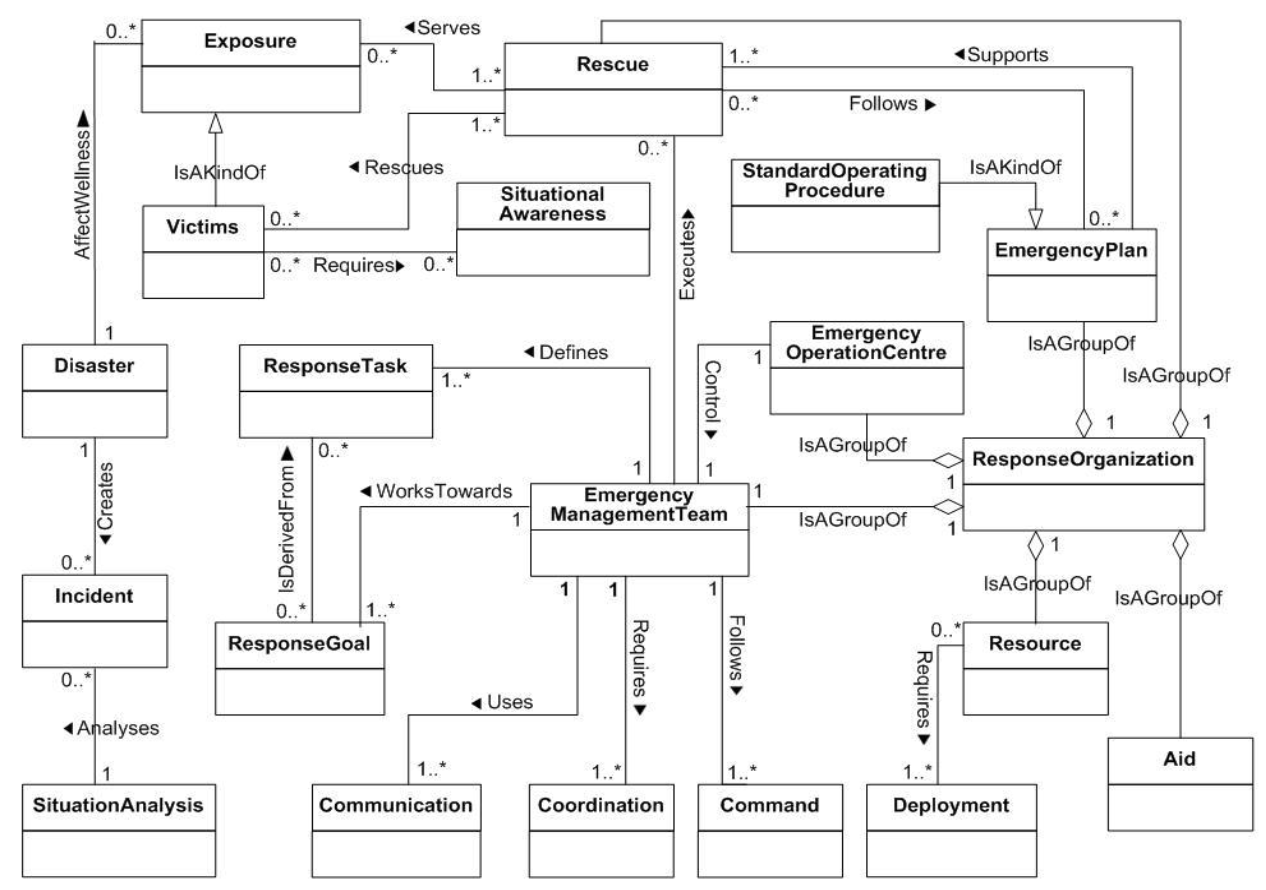
\includegraphics[width=\textwidth]{figures/chap-3/othman-metamodel-response.PNG}
    \caption{Metamodel proposed by \textcite[Fig.4]{othmanDevelopmentValidationDisaster2014} for the response phase of a disaster event.}
    \label{information:othman-metamodel}
\end{figure}

On the other hand, the metamodel proposed by \textcite{benabenMetamodelKnowledgeManagement2016} focuses on collaboration during the response phase.
This metamodel is split into five packages:

\begin{itemize}
    \item Core
    \item Partners
    \item Context
    \item Objectives
    \item Behavior
\end{itemize}

Figure~\ref{information:benaben-metamodel} represents the four main packages: \textbf{Core}, \textbf{Partners}, \textbf{Context} and \textbf{Objectives}.
The \textbf{Behavior} package is excluded as it is solely used to implement a process model of the collaborative behavior using the Business Process Model and Notation (BPMN) representation.
The \textbf{Core} package describes the collaborative process.
This package is composed of five sub-systems: Context, Objectives, Partners, Performance, and Behavior.
Each system represents a specific aspect of collaboration.
These sub-systems correspond to the five previous packages, as each package provides crisis-specific entities to its corresponding sub-system.
The collaboration happens in a given \textit{Context} that contains \textit{Characteristics} and \textit{Threat/Opportunities}.
\textit{Partners} collaborate in this \textit{Context} according to their \text{Resources}, and \text{Capacities} in response to an \text{Event}.
The different \textit{Partners} collaborate towards \textit{Objectives}.
During their collaboration, they review their \textit{Performance} in achieving their \textit{Objectives}.
This package is generic to any collaborative endeavor.
Thus, the metamodel is specified to crises through the surrounding packages.

\begin{figure}[htb]
    \centering
    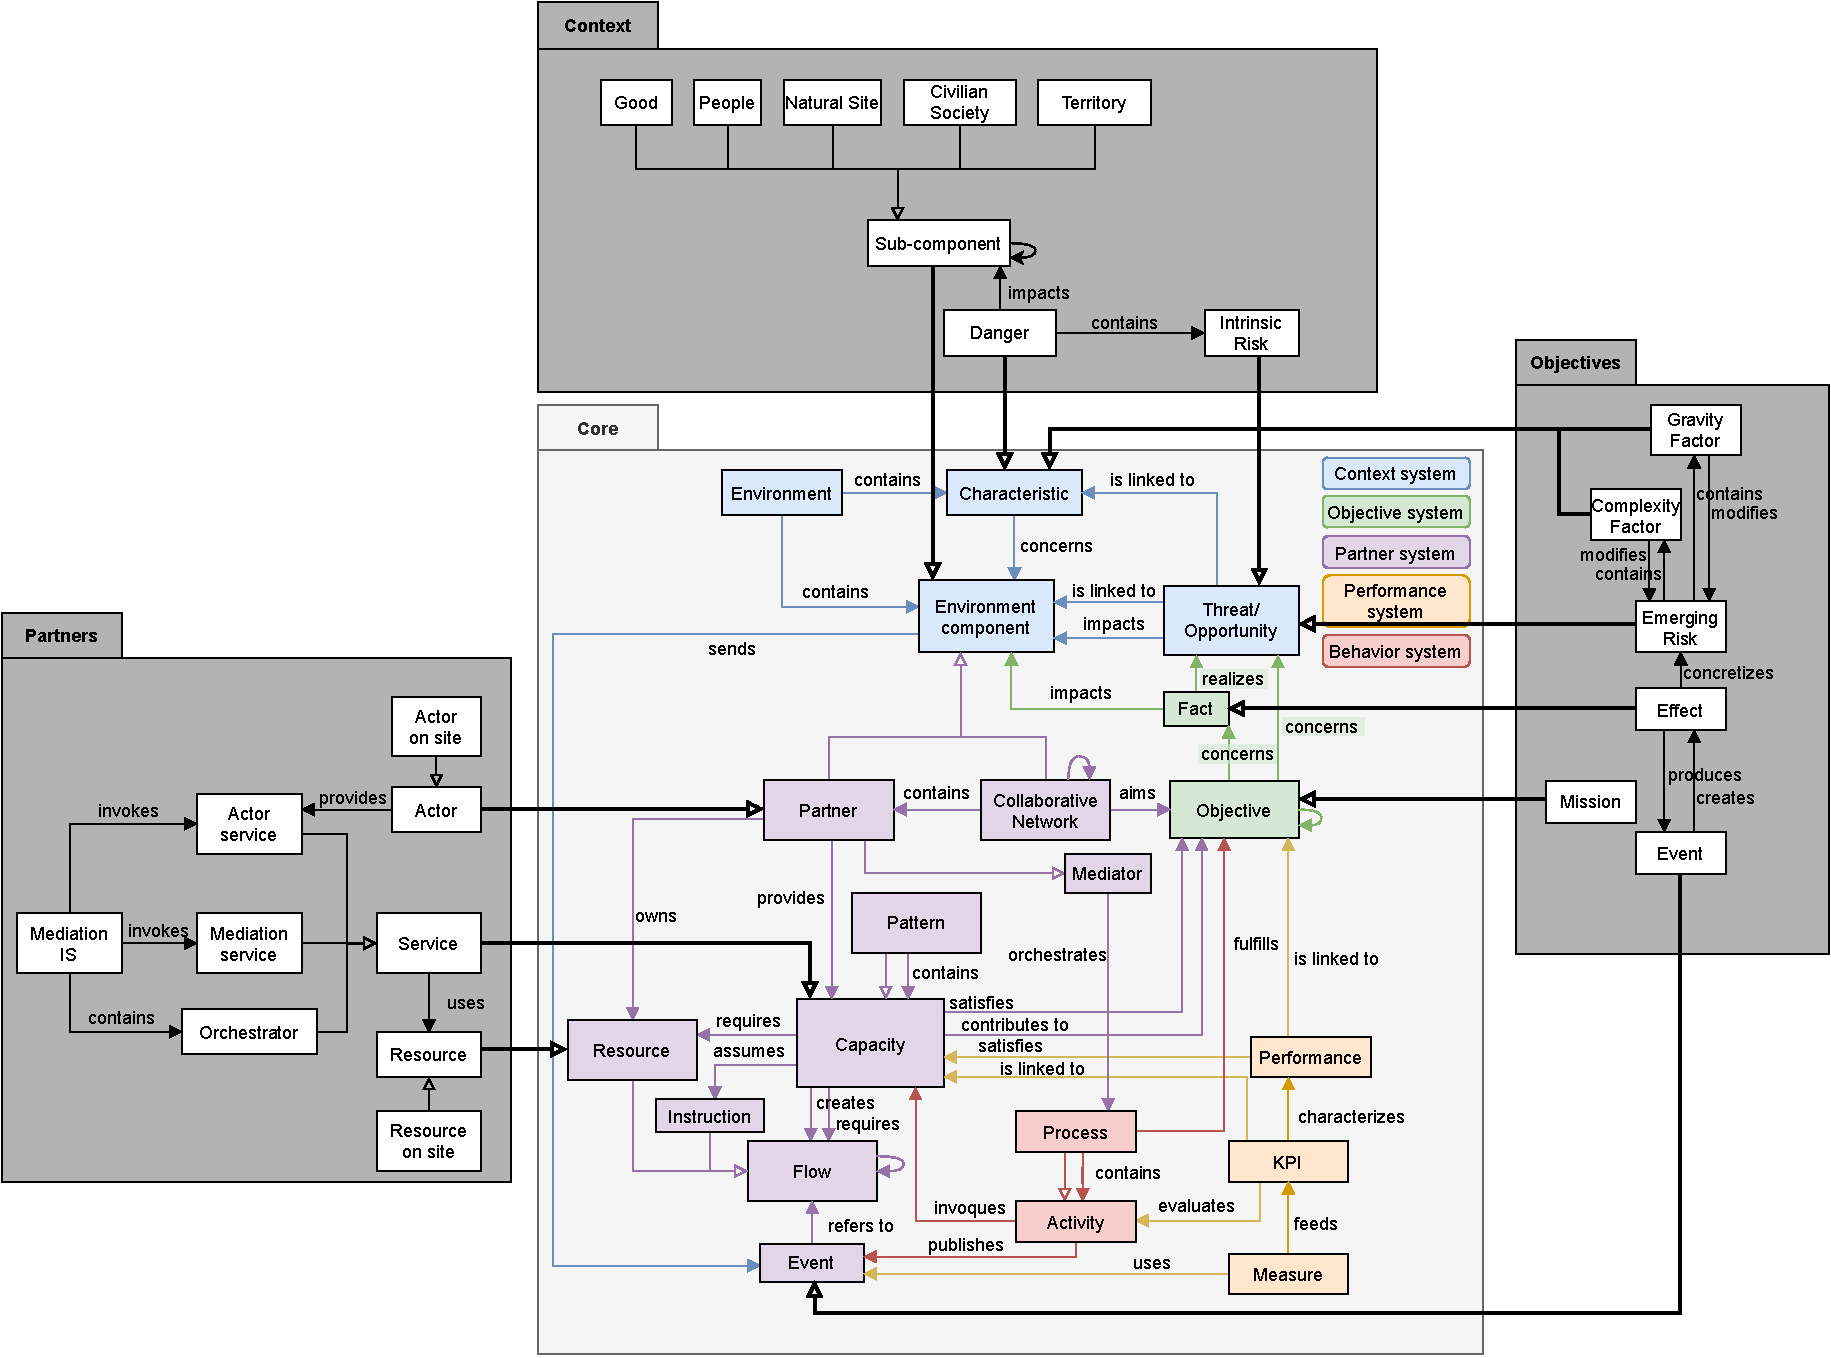
\includegraphics[width=\textwidth]{figures/chap-3/benaben-metamodel-response.pdf}
    \caption{Metamodel proposed by \textcite{benabenMetamodelKnowledgeManagement2016} for the response phase of a disaster event.}
    \label{information:benaben-metamodel}
\end{figure}

The Context package provides additional classes to represent the disaster environment.
It is composed of:
\begin{itemize}
    \item \textit{Good}: human-made elements such as roads, buildings, etc.
    \item \textit{People}: a group of persons
    \item \textit{Natural site}: natural elements such as forest, lake, etc.
    \item \textit{Civilian society}: social actors such as media, institutions, etc.
    \item \textit{Territory}: administrative area such as a county, region, etc.
    \item \textit{Danger}: dangerous characteristics linked to the environment such as seismic area, social instabilities, etc.
    \item \textit{Intrinsic risk}: risk linked to the previous dangers identified which, in the previous example, would correspond to earthquake and riots.
\end{itemize}

The Partners package contains:
\begin{itemize}
    \item \textit{Actor}: emergency responders such as firemen, EMS, etc.
    \item \textit{Resource}: resource used by actors such as a truck, an ambulance for the previous actors
    \item \textit{Service}: capabilities of actors, which correspond to evacuate people and treat injured ones.
    \item \textit{Actor service}: service specifically provided by actors.
    \item \textit{Mediation service}: services provided by the information system used by the partners.
\end{itemize}

The Objectives package:
\begin{itemize}
    \item \textit{Emerging risk}: risk resulting from the event itself (e.g., the collapse of a building, panic, etc.).
    \item \textit{Effect}: a direct consequence of the crisis itself (e.g., 10 injured people, fire, etc.).
    \item \textit{Mission}: objective directly linked to identified risk or effect.
    \item \textit{Event}: event occurring during crisis management that must be considered as triggering an effect.
    \item \textit{Gravity factor}: characteristic of the current situation that may increase or decrease the gravity of the crisis (e.g., rain or wind on a large fire).
    \item \textit{Complexity factor}: characteristic of the current situation that may change the type of the crisis.
\end{itemize}

The objective of both metamodels is to represent the collaboration between the different actors of the response.
However, they differ in their approaches.
On the one hand, the metamodel proposed by \textcite{othmanDevelopmentValidationDisaster2014} is a model that is part of a comprehensive crisis management model.
This model, therefore, seeks to maintain continuity and coherence with the other models, at the cost of less granularity in the description.
It thus focuses essentially on the collaboration between the different actors, leaving aside the description of the context in which this collaboration takes place.
Some entities may appear insufficiently detailed.
For example, the environment is only described by the class \textit{Exposure} and the event through the \textit{Disaster} class.
On the other hand, the model proposed by \textcite{benabenMetamodelKnowledgeManagement2016} focused solely on the response phase of the crisis.
This makes it possible to explore more broadly the information needs of the actors regarding the context.
The modular structure through packages allows specifying each aspect of the crisis.
It allows for a more precise description of essential concepts for Situation Awareness and Actionable Information.
The following presents the identified information, grouping it according to four categories: Actors, Environment, Event, and Collaboration.
The \textbf{Core} package of \textcite{benabenMetamodelKnowledgeManagement2016} is not considered, as its concepts are too abstract for crisis management.
Information from the latter author are shown in \textcolor{magenta}{magenta} and the ones from \textcite{benabenMetamodelKnowledgeManagement2016} are in \textcolor{cyan}{cyan}.

\label{sec:information-si}
\paragraph{Actors}
\begin{itemize}
    \item \textcolor{cyan}{Actor} which includes \textcolor{magenta}{Aid}, \textcolor{magenta}{EmergencyManagementTeam}, \textcolor{magenta}{EmergencyOperationCentre}, \textcolor{magenta}{ResponseOrganization}
    \item \textcolor{cyan}{ActorOnSite} which includes \textcolor{magenta}{Rescue}
    \item \textcolor{cyan}{Resource} which includes \textcolor{magenta}{Resource}
    \item \textcolor{cyan}{ResourceOnSite}
    \item \textcolor{cyan}{Service}
    \item \textcolor{cyan}{ActorService} which includes \textcolor{magenta}{Communication}, \textcolor{magenta}{Coordination}, \textcolor{magenta}{Command}, \textcolor{magenta}{Deployment}, \textcolor{magenta}{SituationAnalysis}
    \item \textcolor{cyan}{MediationService}
\end{itemize}

\paragraph{Environment}
\begin{itemize}
    \item \textcolor{cyan}{Good}
    \item \textcolor{cyan}{People}
    \item \textcolor{cyan}{NaturalSite}
    \item \textcolor{cyan}{CivilianSociety}
    \item \textcolor{cyan}{Territory}
    \item \textcolor{cyan}{Danger}
    \item \textcolor{cyan}{IntrinsicRisk}
\end{itemize}

\paragraph{Event}
\begin{itemize}
    \item \textcolor{cyan}{EmergingRisk} which includes \textcolor{magenta}{Exposure}, \textcolor{magenta}{Victims}
    \item \textcolor{cyan}{Effect} which includes \textcolor{magenta}{Incident}
    \item \textcolor{cyan}{Mission} which includes \textcolor{magenta}{ResponseGoal}
    \item \textcolor{cyan}{Event} which includes \textcolor{magenta}{Disaster}, \textcolor{magenta}{Incident}
    \item \textcolor{cyan}{GravityFactor}
    \item \textcolor{cyan}{ComplexityFactor}
\end{itemize}

\paragraph{Collaboration}
\begin{itemize}
    \item \textcolor{magenta}{EmergencyPlan}
    \item \textcolor{magenta}{StandardOperatingProcedure}
    \item \textcolor{magenta}{ResponseTask}
    \item \textcolor{magenta}{SituationalAwareness}
\end{itemize}

This approach has made it possible to highlight numerous entities that correspond to information manipulated in the response to a crisis.
However, it is also very exhaustive and essentially puts forward information necessary for the computer representation of the situation.
The next section, therefore, overlaps the information needs of an information system, with the ones of decision-makers.

\section{Actionable Information for decision-makers that can be processed automatically}
% * Done
Interviews and meetings with crisis management practitioners have shown that social media handling is currently done mostly manually.
Despite the proven usefulness of this communication channel, it is questionable whether resources should be allocated to such a manual task.
Aware of this issue, some organizations have chosen to delegate it to a third party (VISOV or VOST).
Nevertheless, being able to process the available content on a large scale requires at least partial automation of this processing.
The challenge in automating this processing is to ensure that it does not cause harm instead of solving the original problem.
In particular, the overload of irrelevant or useless information is an issue of such an approach.
The systems developed should require minimal attention from the operators on the menial tasks while keeping them engaged.
This issue leads to this section, which links the information needs of decision-makers with the information needs of crisis management information systems.

The first section of this chapter identified the following information needs:

\begin{itemize}
    \item Location of event, type, cause, and severity.
    \item Environmental conditions (buildings, population density, potential hazards, and their location, etc.).
    \item Information on the response participants (responders already involved, their skills, resources, etc.).
    \item Current and future needs of the responders (number of casualties, their status, etc.).
    \item The available resources for the event (qualified actors, appropriate equipment, etc.).
\end{itemize}

This information helps define the context of the crisis and contributes to the situational awareness of the organization in charge of the response.
As explained in the first section, knowing the context is considered necessary but not sufficient for practitioners to make decisions.
Their primary need is to have access to Actionable Information, on which decisions can be made.
Information is considered Actionable if it meets the following criteria:

\begin{itemize}
    \item is located
    \item is directed to the right role
    \item is timely
    \item is credible
    \item provides context
\end{itemize}

In the case of the information system, some of these criteria are challenging to take into account.
Defining what is the right role to deliver a piece of information or the right time is difficult.
To overcome this problem, the information system must guarantee access to information for as many decision-makers as possible, as soon as possible.
Hence, in the scope of this work, an information is considered actionable if it: i) is located, ii) is credible and iii) provides context.
This information is the information sought by the teams in charge of the response.
It then remains to determine which information that meets the previous criteria can be manipulated by an information system.
This requires an information model capable of representing the information that responders need \parencite{comesBringingStructureDisaster2015}.
These pieces of information are the ones sought by the teams in charge of the response.
It then remains to determine which information that meets the previous criteria can be manipulated by an information system.

Information on the \textbf{Collaboration} is, for instance, not retained in the final model.
This information is used to represent the interactions with the actors and therefore does not meet their needs.
In the same way, the classes \textit{GravityFactor} and \textit{ComplexityFactor} intervening in the representation of the \textbf{Event} are not retained.
These concepts are linked to the functioning of the \textcite{benabenMetamodelKnowledgeManagement2016} metamodel and do not represent directly exploitable information.
Finally, the class \textit{MediationService} in the actor package is not considered since it is linked to the organization's information system.

The final model is then composed of sixteen entities:
\begin{itemize}
    \item \textit{Event}
    \item \textit{Effect}
    \item \textit{Emerging Risk}
    \item \textit{Good}, \textit{People}, \textit{Civilian Society}, \textit{Natural Site} and \textit{Territory} are specific \textit{Environment Components}
    \item \textit{Danger}
    \item \textit{Intrinsic Risk}
    \item \textit{Actor on Site} is a specific \textit{Actor}
    \item \textit{Actor Service}
    \item \textit{Resource on Site} is a specific \textit{Resource}
\end{itemize}

This information model is illustrated in Figure~\ref{information:information-models} and described in the following.

\begin{figure}[htb]
    \centering
    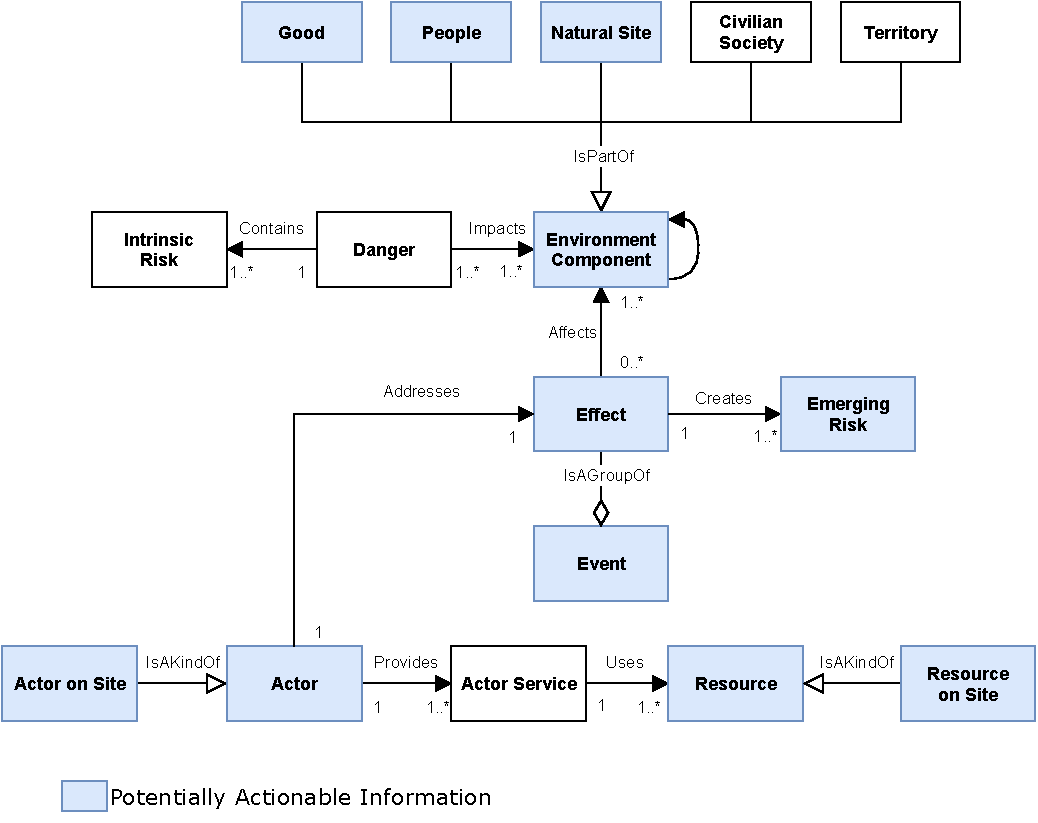
\includegraphics[width=\textwidth]{figures/chap-3/information-needs.pdf}
    \caption{Proposed information model, produced after reviewing the information needed by decision-makers and fitting into an information system for crisis response. The information in \textcolor{blue}{blue} qualifies as Actionable Information.}
    \label{information:information-models}
\end{figure}

It is centered around the concept of \textit{Event}.
The latter is visible through a group of \textit{Effects} it has on the different \textit{Environment Components}.
These \textit{Environment Components} can be either \textit{Good}, \textit{People}, \textit{Civilian Society}, \textit{Natural Site}, or \textit{Territory} entities.
These components are localized on potential \textit{Danger} which contains \textit{Intrinsic Risk}.
These risks can be triggered by the \textit{Event} which creates new \textit{Effects} in their turn (see the relationship between Danger, Risk, and Event proposed in section \hyperref[sec:danger-risk-consequence]{1.1.2.2}).
The consequences of these \textit{Effects} create in their turn new \textit{Emerging Risks} that are potential hazards to the rescue teams.
The latter are represented through the \textit{Actor} entity.
These actors can either be organizations involved in the response or be \textit{Actors on Site} who physically address the \textit{Event}.
Each \textit{Actor} provides a set of skills or services (\textit{Actor Services}).
The skills often require \textit{Resources} that might need to be deployed, in which case they are \textit{Resource on Site}.
Some of this information can be localized and thus qualify as Actionable Information if they match the previous three criteria considered (highlighted in blue in the figure).
There are however, five information from the proposed model that cannot be localized.
An \textit{Actor Service} cannot be localized as it refers to the skills or capabilities (such as the ones proposed by \textcite{othmanDevelopmentValidationDisaster2014} previously).
\textit{Civilian Society} and \textit{Territory} are respectively human organizations (such as a company or media) and geographical entities (such as a state or a region) that are too general to be localized.
A \textit{Danger} refers to an inherent characteristic of the environment that should be identified before an event happens.
This characteristic is also thought to be a wide concept or a geographical area (such as in the example of a seismic zone).
Similarly, \textit{Intrinsic Risks} are latent concepts that do not correspond to a pinpoint on a map.
This information must, therefore, be preferentially identified and located in the crisis environment.
The information identified in this section is reused in the next chapter, which focuses on the automatic collection of some information.

\section*{Conclusion}
The initial objective of this chapter was to identify what information from social media that is relevant to decision-making can be processed automatically.
This question was split into two parts, each of which was addressed in a section.
Each section presented the information needs of decision-makers and the information needs of a crisis management information system, respectively.

The first section is therefore devoted to the processing of social media in organizations responsible for crisis response.
Our first finding is that social media are essentially treated as an auxiliary channel to that of calls and delegated to dedicated operators.
This processing is essentially done manually by these operators or by third parties.
The rest of the first section then presented two concepts adopted in the crisis informatics community: Situational Awareness and Actionable Information.
Situational Awareness refers to the capabilities to perceive, understand and anticipate the state of the environment.
On the other hand, Actionable Information refers to a piece of information that allows immediate decision-making.
In the second part, we have taken the definition of these two concepts and developed how they interact with each other.
In particular, we note that Situational Awareness is a prerequisite for the identification of Actionable Information.
To determine whether a piece of information is actionable, it is first necessary to know the context in which this information is found.
Finally, using interviews conducted and a review of the literature, a set of information that contributes to Situational Awareness and criteria for defining whether the information is actionable were presented.

The second section presented the information needed to implement a crisis model.
Crisis models are computer representations used by information systems to manipulate information.
These representations are necessary to automate the processing of information by the system.
Here, we have examined the two most relevant models in the context of our study.
Then, we have listed all the entities of interest for the automated collection of information.
This list thus forms the second set of information that represents the needs of an information system.

The final section presented the set of information that answers the initial problem: What decision-relevant information from social media can be processed automatically?
To obtain this set, we took each entity in the information system requirements set and looked at whether it met the information needs of the decision-makers.
The result of this filtering led to the model presented in Figure~\ref{information:information-models}.
This model guides the next two chapters.
In the fourth chapter, it is used to define the information that we will try to collect automatically using a semi-supervised algorithm.
This offers the opportunity to create instances of the model's classes automatically.
However, this requires a method capable of detecting information in the social media data.
The next chapter, therefore, proposes a method allowing to automatically extract the required information in the context of crisis management.
The fifth chapter is a proposal for an information system architecture based on similar information models fed by machine learning models.

%%% Local Variables:
%%% mode: latex
%%% TeX-master: "../ma-these.tex"
%%% End: